\chapter{Piani tecnici di processo}

Per lo sviluppo del progetto si utilizzerà un Modello a Spirale: il processo di sviluppo sarà sottoposto in ogni sua fase al rispetto delle quattro task regions offerte da tale modello:
\begin{itemize}
 \item \textbf{Determinazione di obiettivi e alternative}: obiettivi specifici per la fase del progetto
 \item \textbf{Valutazione delle alternative e dei rischi}: analisi dei rischi del progetto; si prendono precauzioni per ridurli o ridurne l’incidenza all’interno del progetto
 \item \textbf{Sviluppo e convalida}: si implementano e si testano le funzionaltà previste
 \item \textbf{Pianificazione}: viene revisionato il progetto e si decide se effettuare un nuovo giro di spirale
\end{itemize}

\begin{figure}[ht]
\centering
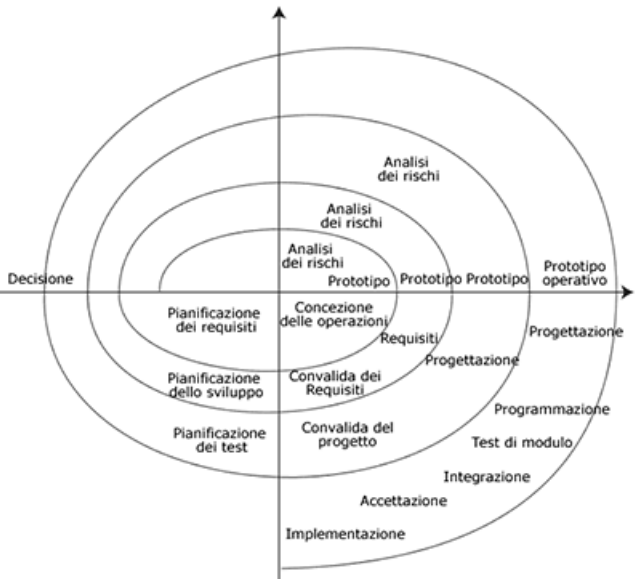
\includegraphics[width=8cm]{img/spirale.png} 
\caption{Meta-modello di sviluppo a spirale}
\label{spiralModel}
\end{figure}

La scelta è ricaduta su questo modello poiché esso rende esplicita la gestione dei rischi e permette di determinare eventuali errori in fasi iniziali.
\paragraph{} In particolare si procederà con un'analisi generica del sistema da realizzare e, successivamente, si eseguiranno almeno due giri di spirale per implementare e testare le funzionalità incrementalmente aggiunte. Alla fine di ogni incremento il sistema deve implementare tutte le funzionalità definite per quel determinato incremento e dev'essere testato completamente.
\paragraph{} La pianificazione del testing avverrà parallelamente rispetto al primo incremento, in modo che alla fine dell'implementazione delle prime funzionalità sia possibile partire subito con il testing e seguire il modello precedentemente descritto.
\paragraph{} Per la specifica delle funzionalità da implementare ad ogni incremento si rimanda all'assegno, mentre per una descrizione approfondita delle stesse si veda il documento di analisi.